% ----------------------------------------------------------------
% AMS-LaTeX Paper ************************************************
% **** -----------------------------------------------------------
\documentclass[11pt]{amsart}
\usepackage{graphicx, mathabx, amssymb,amsfonts,amsmath,amsthm,newlfont}
\usepackage{epsfig,url}
\usepackage{enumerate,enumitem}
\usepackage[colorlinks=true,linkcolor=red,citecolor=blue]{hyperref}
\usepackage[dvipsnames]{xcolor}
\usepackage{color}

\input{aux/commands}

% ----------------------------------------------------------------

\def\abovespace{\vspace{12pt}}
\def\belowspace{\vspace{8pt}}



\addtolength{\hoffset}{-0.0in} \addtolength{\textwidth}{0in}
\addtolength{\voffset}{-0.0in} \addtolength{\textheight}{0.0in}


% -----------------------------------------------------------------

\title{Topological proofs of categorical coherence}

\author{Pierre-Louis Curien}
\address{IRIF, Universit\'e Paris Diderot and $\pi r^2$ team, Inria, France.}
\email{curien@irif.fr}

\author{Guillaume Laplante-Anfossi}
\address{School of Mathematics and Statistics, The University of Melbourne, Victoria, Australia.}
\email{guillaume.laplanteanfossi@unimelb.edu.au}

\date{\today}

\subjclass[2010]{Primary 18N20, Secondary 52B11} 

\keywords{Categorified operads, categorical coherence, Seifert--Van Kampen theorem, polytopes, MacLane coherence theorem, rewriting theory, Morse theory.}

\dedicatory{"We shall construct $KP_n$, as a CW-complex, in Section 2 and show that it is an $(n-1)$-ball. This gives an instant one-step proof of MacLane's theorem in full generality."  \\ --  Mikhail M. Kapranov}

\thanks{The second author was supported by the Andrew Sisson Fund and the Australian Research Council Future Fellowship FT210100256.}

%\thanks{The second author was supported by the European Union's Horizon 2020 research and innovation program under the Marie Sklodowska-Curie grant agreement No 754362 \inlinegraphics{EU.png}, by the Natural Sciences and Engineering Research Council of Canada (NSERC) and by the ANR-20-CE40-0016 Higher Algebra, Geometry and Topology.}


\begin{document}

\begin{abstract}
\correction{We give a short topological proof of coherence for categorified non-symmetric operads by using the fact that the diagrams involved form the 1-skeleton of simply connected CW complexes. 
We also obtain a ``one-step'' topological proof of Mac Lane's coherence theorem for symmetric monoidal categories, as suggested by Kapranov in 1993.  
Our analysis is based on a notion of combinatorial homotopy, which we further study in the special case of polyhedral complexes, leading to a second geometrical proof of coherence which is very close to Mac Lane's original argument.  
We use Morse theory to show that this second method is (strictly) less general than the first.
%we use Morse theory to give a second topological proof which is very close to Mac Lane's original argument. 
We provide a detailed analysis of how  both methods allow us to deduce these two categorical coherence results and discuss possible generalizations to higher categories. }
\end{abstract}

\maketitle



\setcounter{tocdepth}{1}
%\tableofcontents

% !TEX root = ../Coherence.tex

\section*{Introduction} 
\label{s:introduction}

The $n$-dimensional permuto-associahedron, a CW-complex whose faces are in bijection with parenthesized \correction{ordered partitions} of $n+1$ letters, was first introduced by M. Kapranov in his study of higher dimensional Yang--Baxter equations, through the moduli spaces of curves $\overline{\mathcal{M}_{0,n+1}}(\R)$ and the solutions of the Knizhnik--Zamolodchikov equation \cite{kapranov1993}.
It was later realized as a convex polytope by V. Reiner and G. M. Ziegler \cite{reinerCoxeterassociahedra1994}, and more recently through the nested braid fan in \cite{CastilloLiu21}.
%as a simple polytope in \cite{baralicSimplePermutoassociahedron2019} and .

The present note stems from a desire to understand the epigraph, taken from the introduction of \cite{kapranov1993}: what is the precise relationship between the permuto-associahedron and Mac Lane's coherence theorem for symmetric monoidal categories? 
We show that the \emph{simple connectedness} of the former implies the latter, thereby refining and proving Kapranov's claim (see \cref{thm:coherence-MacLane}). 

This is done through a general ``topological coherence theorem" which applies to any simply connected, regular CW complex (\cref{thm:top-coherence}).
\correction{We apply this theorem to another family of polytopes, the operahedra, which encode categorified non-symmetric operads,~\cite{DP15,curienSyntacticAspectsHypergraph2019a,laplante-anfossiDiagonalOperahedra2022a}, yielding a ``one-step'' proof of the associated coherence theorem as well.}

\smallskip

\correction{There is little price to pay, though. For both theorems, we provide a precise bijective correspondence between the 1-skeleton (resp. the 2--cells) on the topological side,  and canonical morphisms (resp. bifunctoriality, naturality, and applications of coherence conditions) on the categorical side (\cref{{bijections-Kapranov},prop:bijection-nestings}). In the case of  permuto-associahedra, we note that their 2-skeleton corresponds to other basic canonical morphisms and coherence conditions than those of Mac Lane (hexagons and naturality of the involutive braiding on one hand versus dodecagons on the other hand), and that the equivalence between these presentations holds true but is  non-trivial (see~\cref{rem:Kapranov-to-MacLane}).  There is also yet another equivalent presentation (and hence yet another proof of coherence), due to Barali\'c, Ivanovi\'c and Petri\'c, that matches the 2-skeleton of a different polytope, which unlike the permuto-associahedron is simple~(see \cref{rem:simple-permutoassociahedron} and \cite{baralicSimplePermutoassociahedron2019}).
}

\smallskip
We also investigate a topological incarnation of Mac Lane's original argument, in the spirit of rewriting theory, see \cref{ss:abstract-rewriting}.  
\correction{We concentrate on  a certain family of simply connected polyhedral complexes endowed with an orientation vector:  the ones \correction{whose outgoing links are all connected} (\cref{p:second-proof}). We show that the orientation vector induces a terminating and confluent rewriting system on  their $1$-skeleton and} obtain  from there another general prood of coherence. In particular, this second theorem can be applied to all polytopes, allowing us to give a second, ``rewriting-theoretic'' proof of both previously mentioned coherence results.  \correction{In the case of operahedra, our rewriting proof simplifies the original proof of Do{\v s}en and Petri{\'c}~\cite{DP15} (see~\cref{rem:DPLA}).}

\correction{It is worth noting that, while general polyhedral complexes admit \emph{abstract} rewriting systems on their sets of vertices,
the families of operahedra  (that include associahedra, encoding non-symmetric monoidal categories) further admit  \emph{term} rewriting systems, which exhibit more structure and are the subject of a companion paper~\cite{CLA24}. In contrast, we shall argue that the abstract rewriting approach to \emph{symmetric} monoidal categories is not informative (see \cref{MacLane-Kapranov-Simple}).}

\smallskip
\correction{Using Morse \correction{theory} on affine cell complexes \cite{bestvinaMorseTheoryFiniteness1997},
 we relate our two approaches by showing that the second is (strictly) less general than the first (\cref{lemma:outgoing-link}).}
 
 \smallskip
Our two general topological coherence theorems can be used to prove other categorical results where polytopes appear, such as coherence for monoidal functors between monoidal categories \cite{epsteinFunctorsTensoredCategories1966}, see \cref{sec:further}.
\correction{They also shed light on some statements in the literature, such as the proof of \cite[Prop.~3.9]{KapranovVoevodsky94}, see\cref{sec:higher}.}
This all points towards further investigation of the relationship between $n$-categorical coherence and $n$-connectedness of appropriate spaces.
\correction{While topological proofs of $2$-categorical coherence already appeared in \cite{Gurski11}, higher dimensional results have been obtained recently by S. Barkan in the context of $\infty$-operads~\cite{barkanArityApproximationInfty2022}}, for which the present results could well be the strict, $n=1$ case.


% !TEX root = ../Coherence.tex

\section{Topological coherence} 
\label{s:polycoherence}

\subsection{Coherence \`a la Van Kampen}

Let $X$ be a regular CW complex, and let $X_k$, $k\geq 0$ denote its $k$-skeleton. 
Let $\mathcal{F}(X)$ be the groupoid with set of objects $X_0$ and morphisms spanned by the following set: for each $x \in X_0$, one identity morphism $\id_x : x \to x$; and for each $1$-cell $\alpha \in X_1$, one morphism $\alpha : x \to y$ oriented according to its attaching map, and one inverse morphism $\alpha^{-1} : y \to x$ in the opposite direction. 
In other words, $\mathcal{F}(X)$ is the free groupoid generated by the morphisms $\alpha$. 
A \emph{combinatorial path} on $X$ is a morphism in $\mathcal{F}(X)$, that is, a composable sequence of $\alpha$ and $\alpha^{-1}$ morphisms (a \emph{word} in $\alpha$ and $\alpha^{-1}$).
Two combinatorial paths $\gamma, \gamma' \in \mathcal{F}(X)(x,y)$ with the same endpoints are said to be \emph{parallel}.

The attaching map of a $2$-cell $A$ of $X$ defines a morphism $\gamma_A \in \mathcal{F}(X)(x,x)$ for a certain $x \in A_0$, given by the sequence of $1$-cells in its image.  
Two parallel combinatorial paths $\gamma, \gamma'$ are said to be \emph{elementary combinatorially homotopic} if they differ exactly by a relation of the form $\gamma_A = \id_x$, for some $2$-cell $A$.
That is, one can rewrite $\gamma$ into $\gamma'$ by replacing some (possibly empty) subword of $\gamma$ with an equivalent subword using the relation $\gamma_A = \id_x$.
More generally, two parallel combinatorial paths are \emph{combinatorially homotopic} if they are related by a sequence of elementary combinatorial homotopies.

%what about the inverses? il faut imposer la relation alpha-1 est inverse de alpha

\begin{thm}
\label{thm:top-coherence}
    Any two parallel combinatorial paths on $X$ are combinatorially homotopic if and only if every path component of $X$ is simply connected.
\end{thm}

\begin{proof}
    Let $\Pi(X)$ denote the fundamental groupoid of $X$, that is the groupoid with objects the vertices of $X$ and morphisms the homotopy classes of paths between them.
    Let $\mathcal{C}(X)$ denote the quotient of the groupoid $\mathcal{F}(X)$ by the relation ``being combinatorially homotopic". 
    Then, we have an isomorphism of groupoids \[ \Pi(X) \cong \mathcal{C}(X) \ . \]
    To show this, one can proceed in three steps. 
    First, one shows that the fundamental groupoid $\Pi(X_1)$ of the $1$-skeleton of $X$ is free on the homotopy classes of maps generated by the attaching maps of the $1$-cells, that is, free on the $\alpha$-morphisms \cite[9.1.5]{Brown2006}.
    Thus, one gets $\Pi(X_1) \cong \mathcal{F}(X)$. 
    Second, one shows that the fundamental groupoid $\Pi(X_2)$ of the $2$-skeleton of $X$ is the free groupoid $\Pi(X_1)$ modulo the relations $\gamma_A=1$, for $A$ a $2$-cell of $X$ \cite[9.1.6]{Brown2006}. 
    This is done through repeated application of the Seifert--Van Kampen theorem; one then has $\Pi(X_2) \cong \mathcal{C}(X)$.
    Third, one shows that the inclusion of $X_2$ in $X$ induces an isomorphism of fundamental groupoids $\Pi(X_2) \cong \Pi(X)$ \cite[9.1.7]{Brown2006}, which concludes the proof of the isomorphism $\Pi(X) \cong \mathcal{C}(X)$.
    The theorem then follows, since every path component of $X$ is simply connected if and only if its fundamental groupoid $\Pi(X)$ is trivial.  
\end{proof}

\subsection{Coherence \`a la Morse}

Let $X\subset \R^n$ be a polyhedral complex, and let $\vec v \in \R^n$ be \emph{generic} on the edges of $X$, meaning that for any pair of vertices $x,y \in X$ belonging to the same edge of $X$, we have $\langle \vec v , x \rangle \neq \langle \vec v, y\rangle$.  
Such a generic vector $\vec v$ induces a natural orientation on the edges of $X$, directed from the source vertex where the functional $\langle \vec v, - \rangle$ is minimal to the target vertex where it is maximal. 

In general, for any face $F \subset X$ of $X$, there is a unique \emph{source} vertex $\so(F)$ such that all its adjacent edges $e \subset F$ are outgoing, and a unique \emph{sink} vertex $\sk(F)$ whose adjacent edges are all incoming.
When the complex $X$ has a unique \emph{global sink}, a vertex whose adjacent edges $e \subset X$ are all incoming, we will denote it by $\sk(X)$. 

Let $H:=\{y \in \R^n \ | \ \langle \vec v , y \rangle = 0\}$ be the linear hyperplane orthogonal to $\vec v$.  
For every vertex $x \in X$, choose $\varepsilon >0$ such that the interval between $\langle \vec v , x \rangle$ and $\langle \vec v , x \rangle + \varepsilon$ does not contain the image of any other vertex under the ``height" function $\langle \vec v, - \rangle$. 

\begin{definition}
    The \emph{outgoing link} of a vertex $x \in X$ is the intersection $\mathcal{F} \cap (H+x+\varepsilon \vec v)$ of the family of faces $\mathcal{F}:=\{ F \subset X \ | \ \so(F)=x \}$ with the affine hyperplane $H+x+\varepsilon \vec v$. 
\end{definition}

A combinatorial path $\gamma$ on $X$ is \emph{oriented} if for any pair $(e, f)$ of consective edges in $\gamma$, we have that $\sk(e)=\so(f)$.  
When no ambiguity arises, we will omit the adjective ``combinatorial" and say only ``oriented path".
Two parallel oriented paths are said to be \emph{elementary combinatorially homotopic} if they are as non-oriented paths. 
They are \emph{combinatorially homotopic} if they are related by a sequence of elementary combinatorial homotopies between oriented paths. 

The following Lemma and its consequence \cref{p:second-proof} translate into topological terms the proof of \cite[Theorem 3.1]{MacLane63}.

\begin{lemma}
\label{l:oriented}
    Let $X$ be a polyhedral complex, and let $\vec v$ be generic on the edges of $X$. 
    If there is a unique global sink $\sk(X)$, then the outgoing link of every vertex is connected if and only if any two parallel oriented paths on $X$ are combinatorially homotopic.
\end{lemma}

\begin{proof}
    We prove the first implication. 
    Suppose that the outgoing link of every vertex is connected. 
    Let $\gamma$ and $\gamma'$ be two parallel oriented paths between two vertices $x$ and $y$. 
    We prove that they are combinatorially homotopic. 
    We proceed by induction on the maximal length $m$ of an oriented path between $x$ and $y$ in $X$. 
    Without loss of generality, we can suppose that $y=\sk(X)$, since if $y\neq\sk(X)$ we can always find an oriented path between $y$ and $\sk(X)$.
    The cases when $m=0$ and $m=1$ are trivial. 
    Suppose that the hypothesis holds up to $m=k-1, k\geq 2$, and consider two paths $\gamma$ and $\gamma'$ for which $m=k$. 
    Let $e$ and $e'$ denote the edges of $\gamma$ and $\gamma'$ that are adjacent to $x$. 
    We examine three cases.
    \begin{enumerate}
        \item If $e=e'$, we can apply the induction hypothesis to $\gamma \setminus e$ and $\gamma' \setminus e'$. 
        \item If $e \neq e'$ and both edges are on the same $2$-face $F$ of $X$, then using the induction hypothesis we have that $\gamma$ and $\gamma'$ are respectively combinatorially homotopic to the paths $\delta$ and $\delta'$ defined as follows: they go from $x=\so(F)$ to $\sk(F)$ by the unique path containing $e$ and $e'$, respectively, and then from $\sk(F)$ to $y$ along the same arbitrary oriented path. 
        Since $\delta$ and $\delta'$ are combinatorially homotopic by definition, the conclusion follows from the transitivity of the combinatorial homotopy equivalence relation. 
        \item Suppose that $e\neq e'$, and that $e$ and $e'$ are \emph{not} on the same $2$-face of $X$. 
        Since the outgoing link of $x$ is connected, there exists a path $\theta$ between $e$ and $e'$ in this link. 
        For every edge $e_i$ of $X$ in the path $\theta$, choose an oriented path $\gamma_i$ in $X$ from $x$ to $y=\sk(X)$ going through $e_i$. 
        Now apply Point (2) above to every pair of parallel oriented paths $(\gamma_i, \gamma_{i+1})$ with $e_i$ and $e_{i+1}$ consecutive in $\theta$, and conclude again by transitivity of the combinatorial homotopy equivalence relation. 
    \end{enumerate}

    In the other direction, suppose that every pair of parallel oriented combinatorial paths are combinatorially homotopic. 
    We show that for any vertex $x$, its outgoing link is connected. 
    Indeed, take two edges $e,e'$ of $X$ with source $x$, and consider their extensions to oriented paths $\gamma, \gamma'$ from $x$ to $\sk(X)$. 
    By hypothesis, these two paths are combinatorially homotopic, that is, there is a sequence of parallel oriented paths from $\gamma$ to $\gamma'$. 
    The collection of first edges in each of these paths defines a path between $e$ and $e'$ in the outgoing link of $x$. 
    Thus, this link is connected. 
\end{proof}

\begin{thm}
\label{p:second-proof}
    Let $X$ be a polyhedral complex, and let $\vec v$ be generic on the edges of $X$.
    Suppose that 
    \begin{enumerate}[label=\roman*)]
        \item there is a unique sink $\sk(X)$, and
        \item the outgoing link of every vertex is connected.
    \end{enumerate}
    Then, any two parallel combinatorial paths on $X$ are combinatorially homotopic.
\end{thm}

\begin{proof} 
    By \cref{l:oriented}, the conclusion holds for \emph{oriented} paths.  
    Let us show that this implies the non-oriented version.
    Let $\gamma$ be a (non-oriented) combinatorial path on $X$ between $x$ and $y$.
    For every vertex $z$ along $\gamma$, one can choose an oriented path $\delta_z$ from $z$ to $\sk(X)$. 
    We observe that for any edge $e: z \to z'$ of $\gamma$, the oriented paths $\delta_z$ and $\delta_{z'}e$ are combinatorially homotopic by hypothesis. 
    Going from $x$ to $y$ inductively one edge at a time and using transitivity of the homotopy equivalence relation, one obtains that $\gamma$ is combinatorially homotopic to $\delta_y^{-1}\delta_x$. 
    Taking another combinatorial path $\gamma'$ parallel to $\gamma$, the same argument shows that $\gamma'$ is combinatorial homotopic to $\delta_y^{-1}\delta_x$.
    Thus $\gamma$ and $\gamma'$ are combinatorially homotopic, which completes the proof. 
\end{proof}

\begin{rem}
    One can consider the abstract rewriting system defined by $\vec v$ on the vertices of $X$, saying that $x$ can be rewritten into $y$ if and only if there is an oriented path from $x$ to $y$ in $X$. 
    The hypotheses of \cref{p:second-proof} impose that this rewriting system is terminating and confluent \cite[Definition 2.1.3]{baaderTermRewritingAll1998}.
\end{rem}

The class of polyhedral complexes to which \cref{p:second-proof} applies is a strict subclass of simply connected complexes, as the following proposition shows.

\begin{proposition}
    \label{lemma:outgoing-link}
    Let $X$ be a polyhedral complex.
    If there is a generic vector $\vec v \in \R^n$ such that the outgoing link of every vertex is connected, then every path component of $X$ is simply connected.
\end{proposition}

\begin{proof}
    Let $\vec v \in \R^n$ be generic with respect to $X$, and suppose that the outgoing link of every vertex is connected. 
    Since $\vec v$ is generic on edges, it defines a Morse function $\langle \vec v , -\rangle$ on $X$, in the sense of \cite[Definition 2.2]{bestvinaMorseTheoryFiniteness1997}.
    As in classical Morse theory, one can determine the homotopy type of $X$ by considering its successive level sets. 
    For $t \in \R$ denote by $X_t$ the closed subspace of $X$ containing points $x$ such that $\langle x, \vec v \rangle$ is at least $t$.
    Let $x$ be a vertex of $X$ of height $h=\langle x, \vec v \rangle$.
    Observe first that $X_{h+\epsilon}$, for some small $\epsilon>0$, is homotopy equivalent to $X_{h'}$ where $h' > h$ is the next greater height at which there is a vertex.
    That is, the homotopy type of $X$ can only change at vertices  \cite[Lemma 2.3]{bestvinaMorseTheoryFiniteness1997}.
    Then, one proves that $X_h$ is homotopy equivalent to the pushout of $X_{h+\epsilon}$ with the cone over the outgoing link of $x$ along the outgoing link of $x$  \cite[Lemma 2.5]{bestvinaMorseTheoryFiniteness1997}.
    By our assumption, the outgoing link of $x$ is connected, and thus the cone over it is simply connected. 
    Since the pushout of simply connected spaces over a connected space is always simply connected (this is an application of the Seifert--Van Kampen theorem), we obtain by induction that every path component of $X$ is simply connected \cite[Point (3) of Corollary 2.6]{bestvinaMorseTheoryFiniteness1997}.
\end{proof}

The converse of \cref{lemma:outgoing-link} is not true in general: many simply connected polyhedral complexes, as the one represented in \cref{fig:outgoingpoly}, have disconnected outgoing links, for many (sometimes for all) choices of generic orientation vectors. 

\begin{figure}[h!]
\centering
\begin{tikzpicture}
    \node[regular polygon,
    draw,
    regular polygon sides = 8, minimum size = 3cm] (p) at (0,0) {};
    \draw[-] (p.202.5)--(180:4)--(p.157.5);
    \draw[-] (p.157.5)--(135:4)--(p.112.5);
    \draw[-] (p.112.5)--(90:4)--(p.67.5);
    \draw[-] (p.67.5)--(45:4)--(p.22.5);
    \draw[-] (p.22.5)--(0:4)--(p.-22.5);
    \draw[-] (p.-22.5)--(-45:4)--(p.-67.5);
    \draw[-] (p.-67.5)--(-90:4)--(p.-112.5);
    \draw[-] (p.-112.5)--(-135:4)--(p.-157.5);
\end{tikzpicture}
\caption{A simply connected polyhedral complex which admits disconnected outgoing links for every choice of generic vector.}
\label{fig:outgoingpoly}
\end{figure}

This implies that the converse of \cref{p:second-proof} does not hold, and thus that MacLane's original proof is far from reaching the full generality of \cref{thm:top-coherence}.
However, it will be sufficient for our purposes, presented in the next Section, since it applies to any polytope.

\begin{proposition}
\label{prop:polytopes}
    Let $P \subset \R^n$ be a polytope, and let $\vec v \in \R^n$ be generic with respect to $P$. 
    Then, $P$ admits a unique sink $\sk(P)$, and
    the outgoing link of every vertex is connected.
\end{proposition}

\begin{proof}
    The existence and uniqueness of a sink is one of the basic, very useful facts about polytopes, see \cite[Theorem 3.7]{Ziegler95}.
    For the second part, we first observe that the \emph{link} of a vertex $x$ in a polytope, called the \emph{vertex figure} and denoted $P/x$, is itself a polytope of dimension $\dim P -1$, whose $(k-1)$-faces are in bijection with the $k$-faces of $P$ that contain $x$ \cite[Proposition 2.4]{Ziegler95}. 
    Now, the affine hyperplane $H+x$, where $H:=\{y \in \R^n \ | \ \langle \vec v, y \rangle = 0\}$, defines a partition of the vertices of $P/x$ into two connected components: the vertices that correspond to incoming, resp. outgoing, edges of $P$ at $x$.
\end{proof}
% !TEX root = ../Coherence.tex

\section{Rewriting method for coherence} 
\label{s:catoperads}







\subsection{Coherence for categorified operads}

Recall from [REF] the definition of the $\mathbb{N}$-colored operad $\mathcal{O}$ encoding ns operads. Its minimal resolution is given by the cellular chains on the operahedra [DEF]. 


\begin{thm}[Coherence theorem] 
\end{thm}

\begin{proof} TBC
\end{proof}

Restricted to categorified ns operad concentrated in arity 1, i.e. to monoidal categories, we recover MacLane's original coherence tbeorem [REF].

There is an analogous statement for weak Cat-operads \cite[Proposition 14.2]{DP15}. In the same fashion as for \cref{thm:equivalenceDPGLA}, one can prove that the two statements are equivalent. 


\subsection{Weak Cat-operads}

\begin{definition}[Weak Cat-operad {\cite{DP15}}]
\end{definition}

\begin{thm} \label{thm:equivalenceDPGLA}
    The data of a categorified ns operad and the data of a weak Cat-operad are equivalent.  
\end{thm}

\begin{proof}
    TBC
\end{proof}




% !TEX root = ../Coherence.tex


%%%%%%%%%%%%%%%%%%%%%%%%%%%%%%%%%%%%%

\subsection{Symmetric monoidal categories} 

We now formulate and prove Mac Lane's coherence theorem for \emph{symmetric} monoidal categories in the same style as above.  Recall that in a symmetric monoidal category, in addition to the natural isomorphisms $\beta$ (with components $\beta_{\kappa,\mu,\nu}:(\kappa\otimes\mu)\otimes\nu\to
\kappa\otimes(\mu\otimes\nu)$), there are natural transformations $\tau$ (with components $\tau_{\mu,\nu}:\mu\otimes\nu\to\nu\otimes\mu$. (Here, we use $\kappa,\mu,\nu,\ldots$ range over the objects of the category, consistently with the notation used in *** Sections 2.1 and 2.2 ***.)
In addition to  the pentagons (described by replacing $\circ$ with $\otimes$ in the first pentagon in~\cref{def:catoperad}), there are hexagons (for all objects $\kappa,\mu,\nu$):
\begin{center}
\resizebox{0.5\linewidth}{!}{
    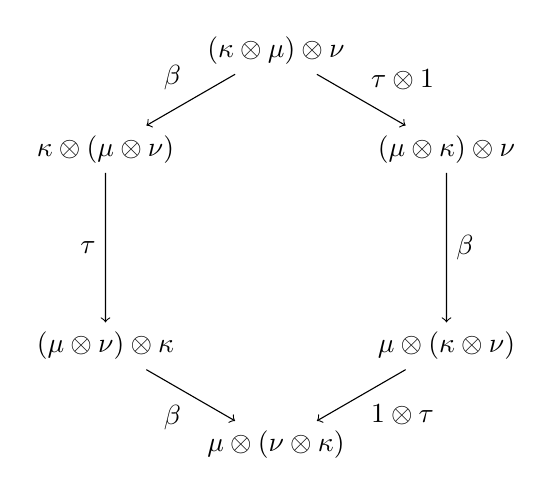
\begin{tikzpicture}[scale=2.5]
    \node (P1) at (0,1) {$(\kappa\otimes \mu) \otimes \nu$};
    \node (P2) at (-0.866,0.5) {$\kappa\otimes (\mu \otimes \nu)$};
    \node (P3) at (-0.866,-0.5) {$(\mu \otimes \nu) \otimes \kappa$};
    \node (P4) at (0,-1) {$\mu \otimes (\nu \otimes \kappa)$};
    \node (P5) at (0.866,0.5) {$(\mu \otimes \kappa) \otimes \nu$} ;
    \node (P6) at (0.866,-0.5) {$\mu \otimes (\kappa \otimes \nu)$};
    \draw[->] (P1)--(P2) node[midway,above left] {$\beta$};
    \draw[->] (P2)--(P3) node[midway,left] {$\tau$};
    \draw[->] (P3)--(P4) node[midway,below left] {$\beta$};
    \draw[->] (P1)--(P5) node[midway,above right] {$\tau\otimes 1$};
    \draw[->] (P5)--(P6) node[midway,right] {$\beta$};
    \draw[->] (P6)--(P4) node[midway,below right] {$1\otimes\tau$};
\end{tikzpicture}
}
\end{center}


We construct the free symmetric monoidal category on a set $S$.
We define a small category $\mathcal{S}^{\mathrm{ML}}$ whose set ${\cal T}_S$  is  given by the following rules:
\begin{enumerate}
    \item if $a \in S$, then $a\in{\cal T}_S$;
    \item if $t_1 \in {\cal T}_S$ and $t_2 \in {\cal T}_S$, then $t_1 \otimes t_2\in{\cal T}_S$.
\end{enumerate}
We call the elements of $S$ generating objects.

Now we define a set $M^{\mathrm{ML}}$ of basic morphisms $\beta: (t_1 \otimes t_2) \otimes t_3 \leftrightarrow t_1 \otimes (t_2\otimes t_3) : \beta^{-1}$  and $\tau: t_1\otimes t_2 \leftrightarrow t_2 \otimes t_1 : \tau^{-1}$,  for every $t_1,t_2,t_3  \in {\cal T}_S$
.
We then define the generating morphisms of  $\mathcal{S}^{\mathrm{ML}}$ by the following rules:
\begin{enumerate}
    \item if $\phi \in M^{\mathrm{ML}}$, then $\phi$ is a generating morphism; 
    \item if $\phi : t_1 \to t_2$ is a generating morphism and $t_3 \in {\cal T}_S$, then $\phi \otimes \id : t_1 \otimes t_3 \to t_2 \otimes t_3$ and $\id \otimes \phi : t_3 \otimes t_1 \to t_3 \otimes t_2$ are generating morphisms.
\end{enumerate}
We then define $\mathcal{S}^{\mathrm{ML}}$ as the free category over all generating morphisms. 
This finishes the construction of the category $\mathcal{S}^{\mathrm{ML}}$.

\begin{definition}
    We denote  by $\mathcal{F}(S)$ the quotient of $\mathcal{S}^{\mathrm{ML}}$ by localization (inverting the $\beta$ and $\tau$ morphisms), the axioms of bifunctors, the naturality conditions for $\beta$ and $\tau$, and the coherence diagrams defining   symmetric monoidal categories.
    \end{definition}

We obtain that $\mathcal{F}(S)$ is the free  symmetric monoidal category on $S$. 
That is, for any symmetric monoidal category $\mathcal{C}$, and for any function $\rho : S \to \obj(\mathcal{C})$, there is a unique \emph{strict} morphism of symmetric monoidal categories $\mathcal{F}(S) \to \mathcal{P}$ which extends $\rho$. It sends the formal basic morphisms to the actual canonical morphisms of $\mathcal{C}$.
By precomposing it with the quotient map $[-]:\mathcal{S}^{\mathrm{ML}} \to \mathcal{F}(S)$, we get  functor $\extd{-}{\mathrm{ML}}:\mathcal{S}^{\mathrm{ML}} \to \mathcal{C}$.

\smallskip
It turns out that Kapranov's topological proof is not based on the above presentation of $\mathcal{F}(S)$, but  on another presentation of this category, that is made explicit in~\cite{baralicSimplePermutoassociahedron2019}. 
We recall this presentation. We define another category $\mathcal{S}^{\mathrm{K}}$ as follows. Its objects are the same as those of $\mathcal{S}^{\mathrm{ML}}$. We define a set $M^{\mathrm{K}}$ of basic morphisms $\beta: (t_1 \otimes t_2) \otimes t_3 \leftrightarrow t_1 \otimes (t_2\otimes t_3) : \beta^{-1}$ for every $t_1,t_2,t_3  \in {\cal T}_S$ , and $\tau: a\otimes b \leftrightarrow b \otimes a : \tau^{-1}$ for every $a,b  \in S$, i.e., we \emph{limit $\tau$ to generating objects}.
Generating morphisms are defined in the same way as for $\mathcal{S}^{\mathrm{ML}}$.
We note that by construction $\mathcal{S}^{\mathrm{K}}$ is a wide subcategory of $\mathcal{S}^{\mathrm{ML}}$.

\begin{definition}
    We denote   by $\mathcal{F}(S)^{\mathrm{K}}$ the quotient of $\mathcal{S}^{\mathrm{K}}$ by localization (inverting the $\beta$ and $\tau$ morphisms), the axioms of bifunctors, the naturality conditions for $\beta$, and the coherence diagrams defining   monoidal categories  and by the  axioms in dodecagonal form (for $a,b,c$ ranging on $S$ only) given by the solid arrows in~\cref{fig:dodecagon}.
\end{definition}
\begin{figure}[h!]
\begin{center}
\resizebox{0.8\linewidth}{!}{
 \begin{tikzpicture}[scale=6.5]
    \node (P1) at (0,1) {$(a \otimes b) \otimes c$};
    \node (P2) at (-0.5,0.866) {$a \otimes (b \otimes c)$};
    \node (P3) at (-0.866,0.5) {$a \otimes (c \otimes b)$};
    \node (P4) at (-1,0) {$(a \otimes c) \otimes b$};
    \node (P5) at (-0.866,-0.5) {$(c \otimes a) \otimes b$} ;
    \node (P6) at (-0.5,-0.866) {$c \otimes (a \otimes b)$};
    \node (P7) at (0,-1) {$c \otimes (b \otimes a)$};
    \node (P8) at (0.5,-0.866) {$(c \otimes b) \otimes a$};
    \node (P9) at (0.866,-0.5) {$(b \otimes c) \otimes a$};
    \node (P10) at (1,0) {$b \otimes (c \otimes a)$};
    \node (P11) at (0.866,0.5) {$b \otimes (a \otimes c)$} ;
    \node (P12) at (0.5,0.866) {$(b \otimes a) \otimes c$};
    \draw[->] (P1)--(P2) node[midway,above left] {$\beta$};
    \draw[->] (P2)--(P3) node[midway,above left] {$1\otimes\tau$};
    \draw[->] (P3)--(P4) node[midway,above left] {$\beta^{-1}$};
    \draw[->] (P4)--(P5) node[midway,below left] {$\tau\otimes 1$};
    \draw[->] (P5)--(P6) node[midway,below left] {$\beta$};
    \draw[->] (P6)--(P7) node[midway,below left] {$1\otimes\tau$};
    \draw[->] (P1)--(P12) node[midway,above right] {$\tau\otimes 1$};
    \draw[->] (P12)--(P11) node[midway,above right] {$\beta$};
    \draw[->] (P11)--(P10) node[midway,above right] {$1\otimes\tau$};
    \draw[->] (P10)--(P9) node[midway,below right] {$\beta^{-1}$};
    \draw[->] (P9)--(P8) node[midway,below right] {$\tau\otimes 1$};
    \draw[->] (P8)--(P7) node[midway,below right] {$\beta$};
    \draw[->,dashed] (P2)--(P9) node[midway,above right] {$\tau$};
    \draw[->,dashed] (P3)--(P8) node[midway,below left] {$\tau$};
\end{tikzpicture}
\quad\quad
 \begin{tikzpicture}[scale=6.5]
    \node (P1) at (0,1) {$(\set{a}  \set{b})  \set{c}$};
    \node (P2) at (-0.5,0.866) {$\set{a}  (\set{b}  \set{c})$};
    \node (P3) at (-0.866,0.5) {$\set{a}  (\set{c}  \set{b})$};
    \node (P4) at (-1,0) {$(\set{a}  \set{c})  \set{b}$};
    \node (P5) at (-0.866,-0.5) {$(\set{c}  \set{a})  \set{b}$} ;
    \node (P6) at (-0.5,-0.866) {$\set{c}  (\set{a}  \set{b})$};
    \node (P7) at (0,-1) {$\set{c}  (\set{b}  \set{a})$};
    \node (P8) at (0.5,-0.866) {$(\set{c}  \set{b})  \set{a}$};
    \node (P9) at (0.866,-0.5) {$(\set{b}  \set{c})  \set{a}$};
    \node (P10) at (1,0) {$\set{b}  (\set{c}  \set{a})$};
    \node (P11) at (0.866,0.5) {$\set{b}  (\set{a}  \set{c})$} ;
    \node (P12) at (0.5,0.866) {$(\set{b}  \set{a})  \set{c}$};
    \node (P13) at (0,0) {$\set{a,b,c}$} ;
    \draw[-] (P1)--(P2) node[midway,above left] {$\set{a}\set{b}\set{c}$};
    \draw[-] (P2)--(P3) node[midway,above left] {$\set{a}\set{b,c}$};
    \draw[-] (P3)--(P4) node[midway,above left] {$\set{a}\set{c}\set{b}$};
    \draw[-] (P4)--(P5) node[midway,below left] {$\set{a,c}\set{b}$};
    \draw[-] (P5)--(P6) node[midway,below left] {$\set{c}\set{a}\set{b}$};
    \draw[-] (P6)--(P7) node[midway,below left] {$\set{c}\set{a,b}$};
    \draw[-] (P1)--(P12) node[midway,above right] {$\set{a,b}\set{c}$};
    \draw[-] (P12)--(P11) node[midway,above right] {$\set{b}\set{a}\set{c}$};
    \draw[-] (P11)--(P10) node[midway,above right] {$\set{b}\set{a,c}$};
    \draw[-] (P10)--(P9) node[midway,below right] {$\set{b}\set{c}\set{a}$};
    \draw[-] (P9)--(P8) node[midway,below right] {$\set{b,c}\set{a}$};
    \draw[-] (P8)--(P7) node[midway,below right] {$\set{c}\set{b}\set{a}$};
\end{tikzpicture}} 

\end{center}
\caption{Kapranov dodecagons}
\label{fig:dodecagon}
\end{figure}

We pause here to reflect on the difference between the two presentations. In the second, we have less generators, and we have lost hexagons. For an intuition, here is how Mac Lane himself motivated his hexagonal axioms (verbatim, just changing the notation to fit with ours) in~\cite{MacLane63}:

\begin{quote}
The instance $\tau_{\kappa\otimes \mu,\nu}$ interchanges the block $\kappa\mu$ with the single letter $\nu$; the hexagon condition states that this interchange may be replaced by two instances of $\tau$ which interchange single letters with $\nu$. Repeated such replacement using instances of the hexagon shows that any interchange of successive blocks may be replaced by interchanges of successive letters.
\end{quote}

In other words, hexagons are now taken as definitions rather than axioms. But how do we guarantee that the  general $\tau$ morphisms defined in this way define a natural transformation? This is what the dodecagons are for, as we shall see.

\smallskip
Let $\mathcal{C}$  be a symmetric monoidal category. Then by freeness  $\rho : S \to \obj(\mathcal{C})$, $\rho$ extends uniquely to a functor $\extd{-}{\mathrm{K}}:\mathcal{S}^{\mathrm{K}} \to \mathcal{C}$.
This functor is the restriction of $\extd{-}{\mathrm{ML}}$ to $\mathcal{S}^{\mathrm{K}}$.
In the next proposition, we  establish ``Kapranov style'' coherence.



\begin{proposition}
\label{thm:coherence-Kapranov}
    For any symmetric monoidal category $\mathcal{C}$, for any  function $\rho : S \to \obj(\mathcal{C})$, and for any two parallel morphisms $\phi_1,\phi_2: t_1 \to t_2$ in~$\mathcal{S}^{\mathrm{K}}$, we have $\extd{\phi_1}{\mathrm{K}}=\extd{\phi_2}{\mathrm{K}}$.
\end{proposition}
\begin{proof}
The conclusion will readily follow from the following two properties
\begin{enumerate}
\item[(1)] If $\phi_1,\phi_2: t_1 \to t_2$ in~$\mathcal{S}^{\mathrm{K}}$, then $[\phi_1]^{\mathrm{K}}=[\phi_2]^{\mathrm{K}}$, where $[-]^{\mathrm{K}}:\mathcal{S}^{\mathrm{K}}\to  \mathcal{F}(S)^{\mathrm{K}}$ is the quotient functor.  
\item[(2)] The relations in Kapranov presentation are valid in $\mathcal C$.
\end{enumerate} 
Indeed, (2) says that $\extd{-}{\mathrm{K}}$ factors through $[-]^{\mathrm{K}}$, hence the statement is reduced to proving (1).

The proof of  (2) is visualised in~\cref{fig:dodecagon} (left part).  The two dotted lines delimit two Mac Lane hexagons on the top and at the bottom and a naturality square in the middle (explicitly, the two dotted $\tau$ morphisms are $\tau_{a,b\otimes c}$ and $\tau_{a,c\otimes b}$. 

 We prove (1) as an application of our general theory of~\cref{s:polycoherence}, like in the categorified operadic case. Again, we  exhibit  a bijective correspondence between the $i$-dimensional faces of Kapranov's poset ${\mathcal P}$ (realised later as a polytope in~\cite{reinerCoxeterassociahedra1994}), for $0\leq i\leq 2$, and the data defining $\mathcal{S}^{\mathrm{K}}$.  We start by presenting this poset. We fix a finite  subset $A\inc S$ of generating objects. 
 An element of $P$ is a (non necessarily fully) parenthesised word whose letters are finite non-empty subsets of $A$ forming a partition of $A$.  For example, with $A=\set{a_1,\ldots,a_6,a_7}$, the following is a face:
 $$\begin{array}{l}
 (\set{a_1} \set{a_4} \set{a_2,a_6}) \set{a_3,a_5,a_7}
 \end{array}$$
The elements of $P$ can be drawn as planar trees whose leaves are decorated with subsets of $A$ forming together a partition of $A$.  The subface relation $\prec$ is defined by two clauses: one can contract an edge of the tree (or remove a node all of whose  incoming edges are leaves and decorate its outcoming edge -- now a leaf- with the union of the decorations of those incoming edges, as illustrated below:
$$\begin{array}{lll}
 (\set{a_1} \set{a_4} \set{a_2,a_6}) \set{a_3,a_5,a_7} & \prec & \set{a_1} \set{a_4} \set{a_2,a_6} \set{a_3,a_5,a_7} \\
 (\set{a_1} \set{a_4} \set{a_2,a_6}) \set{a_3,a_5,a_7} & \prec &  \set{a_1,a_2,a_4,a_6} \set{a_3,a_5,a_7}
 \end{array}$$
 The maximum face is $A$.
These posets, parametrized by $A$, have been realized by CW-complexes (resp. by polytopes) in \cite{kapranov1993} (resp. \cite{reinerCoxeterassociahedra1994}).
The 0-dimensional faces of $P$ are fully parenthesized words whose letters are singletons, and are in obvious bijective correspondence with the elements of ${\cal T}_A$ in which each generating object occurs exactly once (as in all coherence conditions).  The 1-dimensional faces are 
\begin{itemize}
\item
either fully parenthesised words whose letters are singletons but for one letter which is a two element set $\set{a_i,a_j}$ and feature a generating morphism whose underlying basic morphism is $\tau_{a_i,a_j}$, 
\item or an ``almost'' fully parenthesised word of singletons, with just one parenthesis removed, yielding a subword $\set{a_i,a_j,a_k}$, featuring an application of the basic morphism $\beta_{a_i,a_j,a_k}$ or $\beta_{a_i,a_j,a_k}^{-1}$
-- the orientation being ``decided'' by	 the shape of the end vertices.
\end{itemize}
Finally, the 2-dimensional faces can be analysed much in the same way as in  ***Proposition 2.6 ***, and seen to correspond to bifunctoriality, naturality of $\beta$, and to the pentagons and dodecagons. We have picture the poset view of the 
latter in~\cref{fig:dodecagon} (right part).
\end{proof}

The following proposition seems unrelated to coherence issues, but in fact its proof relies on the  coherence result that we just established.
\begin{proposition} \label{Kapranov-MacLane}
The identity-on-objects  functor from  $\mathcal{F}(S)^{\mathrm{K}}$ to 
$\mathcal{F}(S)$ that maps $[\psi]^{\mathrm{K}}$ to $[\psi]$ is an isomorphism of categories.
\end{proposition}

\begin{proof}
We first note that it follows from (2) in the proof of~\cref{thm:coherence-Kapranov} (applied to $\mathcal{F}(S)$) that the map in the statement is well defined. We build a map in the converse direction.
 For each morphism $\phi\in\mathcal{S}^{\mathrm{ML}}$, there exists a morphism $\psi\in\mathcal{S}^{\mathrm{K}}$ such that $[\phi]=[\psi]$. Such a morphism can be obtained by repeatedly applying the procedure described in the above quotation of Mac Lane.  We define a candidate for being an inverse of the map in the statement by mapping $[\phi]$ to $[\psi]^{\mathrm{K}}$. We show that this  map is well-defined. Indeed, if  a morphism $\phi'$ of  $\mathcal{S}^{\mathrm{ML}}$ is such that $[\phi]=[\phi']$ and if $\psi'$ is a morphism of $\mathcal{S}^{\mathrm{K}}$ such that $[\phi]=[\psi']$, then a fortiori $\psi$ and $\psi'$ are parallel, and hence by (1) in the proof of~\cref{thm:coherence-Kapranov}, we get  $[\psi]^{\mathrm{K}}=[\psi']^{\mathrm{K}}$. 
 Finally, starting from  $[\phi]\in\mathcal{F}(S)$, applying the two maps successively returns  $[\psi]$ which is equal to $[\phi]$ by construction. In the other direction, starting from $[\psi]^{\mathrm{K}}$, we get $[\psi]$ and  we have nothing to do to pick a representative from $\mathcal{S}^{\mathrm{K}}$, so that applying the two maps does nothing either.
\end{proof}

\begin{thm}[Coherence theorem]
\label{thm:coherence-MacLane}
    For any symmetric monoidal category $\mathcal{C}$, for any  function $\rho : S \to \obj(\mathcal{C})$, and for any two parallel morphisms $\phi_1,\phi_2: t_1 \to t_2$ in~$\mathcal{S}^{\mathrm{ML}}$, we have $\extd{\phi_1}{\mathrm{ML}}=\extd{\phi_2}{\mathrm{ML}}$.
\end{thm}
\begin{proof} 
If $\phi_1$ and $\phi_2$ are parallel in $\mathcal{S}^{\mathrm{ML}}$, then by~\cref{Kapranov-MacLane}
there exist $\psi_1$ and $\psi_2$ in $\mathcal{S}^{\mathrm{K}}$ such that $[\psi_1]=[\phi_1]$ and 
$[\psi_2]=[\phi_2]$
 (in particular $\psi_1$ and $\psi_2$ are parallel).
Then we have  
$$\extd{\phi_1}{\mathrm{ML}} = \extd{\psi_1}{\mathrm{ML}}= \extd{\psi_1}{\mathrm{K}} 
=  \extd{\psi_2}{\mathrm{K}} 
 =  \extd{\psi_2}{\mathrm{ML}}  =  \extd{\phi_2}{\mathrm{ML}}$$ 
 where the equality in the middle 
follows from~\cref{thm:coherence-Kapranov}.
\end{proof}

%{\color{blue} OBSOLETE
%One can use the same ideas to prove MacLane's coherence theorem for \emph{symmetric} monoidal categories, using the family of permutoassociahedra \cite{kapranov1993,reinerCoxeterassociahedra1994,baralicSimplePermutoassociahedron2019,CastilloLiu21}. 
%Here we simply formulate the theorem, the proof is really the same as the one of \cref{thm:coherence-operahedra}.
%
%Let $W_n$ denote the set of non-commutative, fully parenthesized words on $n$ distinct letters. 
%Let $(\mathcal{C}, \otimes)$ be a symmetric monoidal category.
%Each $w \in W_n$ defines in an obvious way a functor $[w] : \mathcal{C}^{\times n} \to \mathcal{C}$.
%For instance, if $w=((ab)c)(ed)$, then the associated functor is defined on objects and morphisms by the formula
%\begin{eqnarray*}
%    [w] \quad : \quad \mathcal{C}^{\times n} & \to & \mathcal{C} \\
%    (a,b,c,d,e) & \mapsto & ((a \otimes b) \otimes c)\otimes (e \otimes d) \ .
%\end{eqnarray*}
%We consider the free category $\mathcal{W}_n$ which has objects the elements of $W_n$, and morphisms generated by the ones of the form $\phi : w_1 \to w_2$, where the word $w_2$ is obtained from $w_1$ by applying either $\alpha : ((ww')w'') \to (w(w'w''))$, $\alpha^{-1}$, or $\tau : ww' \to w'w$ to a subword of $w_1$.
%To any such $\phi$ one can associate a natural transformation $[\phi] : [w_1] \to [w_2]$ in $\mathcal{C}$ in the obvious way. 
%
%\begin{thm}[MacLane's coherence theorem]
%    \label{thm:MacLanesym}
%    For any symmetric monoidal category $\mathcal{C}$, and for any pair of parallel morphisms $\phi_1,\phi_2: w_1 \to w_2$ in $\mathcal{W}=\{\mathcal{W}_n\}_{n\geq 1}$, we have $[\phi_1]=[\phi_2]$.
%\end{thm}}










%\begin{rem}
%\label{rem:29}
%MacLane's original proof \cite{MacLane63} proceeds in two stages, (anachronically) much like the one of Do{\v s}en--Petri{\'c} for weak Cat-operads (\cref{rem:DPLA}).
%But the second proof of \cref{thm:coherence-operahedra} suggests a one stage proof: indeed, fixing a total order on the letters, allowing $\tau: ab \to ba$ only if the maximal letter is in $a$ (and adding $\tau^{-1}$), we get a terminating and confluent rewriting system. 
%\end{rem}


% !TEX root = ../Coherence.tex

\section{Perspectives}


\Guillaume{Flow categories?}


\subsection{Rewriting theory and Koszul duality}
Any generic vector $\vec v$ defines a canonical rewriting system on the vertices of a polyhedral complex $X$, which is moreover always terminating and confluent. 
The confluence of the rewriting system described in the second proof of \cref{thm:coherence-operahedra} can be used to give a proof that the colored operad $\mathcal{O}$ \cite[Definition 4.2]{laplante-anfossiDiagonalOperahedra2022a} encoding non-symmetric operads is Koszul (and which avoids resorting to the diamond lemma!): one can proceed with the rewriting method \cite[Section 8.3]{LodayVallette12} adapted to colored operads \cite{KhariKhoro20}, along the lines of the Remark following \cite[Theorem 9.1.5]{LodayVallette12}. 

In the other way around, one can use the fact that $\mathcal{O}$ is Koszul to prove the coherence theorem for categorified non-symmetric operads, using \cite[Theorem 15]{marklCoherenceConstraintsOperads2001} in a suitable generalization of \cite[Example 16]{marklCoherenceConstraintsOperads2001}.
Thus, the categorical coherence theorem for $\mathcal{O}$-algebras and the fact that $\mathcal{O}$ is Koszul are equivalent.
Considering the large scope of the theory developed in \cite{marklCoherenceConstraintsOperads2001}, this could be a general fact. 

\Guillaume{Application to Drinfeld}
\Guillaume{Morse theory and rewriting; polygraphs, higher dimensional rewriting?}

\subsection{Higher categories} 
\label{sec:higher}
\cref{thm:top-coherence} demonstrates that, in the case of monoidal categories, coherence is equivalent to the vanishing of the first homotopy groups of the associahedra. 
Since the associahedra are contractible, and therefore all their homotopy groups vanish, one could hope for a topological proof of higher dimensional coherence theorems.
Seeing a monoidal category as a bicategory with one object, one can ask about a coherence theorem for tricategories with one object. 
A first look at the diagrams in the beginning of \cite[Section 2]{gordonCoherenceTricategories1995} suggests that such a theorem should be at least related to the vanishing of the second homotopy groups of the associahedra.  
To formulate higher dimensional statements, one needs a good structure of pasting scheme on each associahedron, which is the subject of ongoing work \cite{AMMLA}. 

Recent results of S. Barkan provide evidence for these higher dimensional statements, in the context of $\infty$-operads \cite{barkanArityApproximationInfty2022}.
In this vein, it seems likely that the present results could be interpreted as a strict version and a special case of \cite[Theorem B]{barkanArityApproximationInfty2022}. 
It would be interesting to see how the permutoassociahedra arise in the strictification process, and how they are related to operadic partition complexes.  




\bigskip

\emph{Acknowledgements.}   
We would like to thank all the participants of the Roberta Seminar held on September 30th, 2020 in Paris for planting the seeds of the present note.  
We would like to thank Andrea Bianchi for enlightening discussions, for pointing out mistakes in a first draft, and for reminding us of the Seifert--Van Kampen theorem. 
Finally, we are grateful to Zoran Petri{\'c} for precious discussions on weak Cat-operads, to Marcy Robertson \correction{and to the anonymous referee} for helpful comments \correction{which led to substantial improvements of the paper}.
\correction{
The first author wishes to thank the Mathematisches Forschungsinstitut Oberwolfach for several visits as a Research Fellow in 2020 and 2021, thanks to which much of the work presented here, as well as in the companion paper \cite{CLA24}, could take off.
The second author would like to thank the Copenhagen Center for Geometry and Topology as well as the Max Planck Institute for Mathematics in Bonn where part of this work was carried out.}


\bibliographystyle{amsalpha}

\bibliography{Coherence}


\end{document}



